%%% fs-state-consistency - Fault tolerance

\label {fs-consistency-section}

In the previous section, we demonstrated how state-of-the-art stream processing systems handle non-deterministic behavior in order to achieve~ exactly-once. All these systems make state recoverable before output elements which depend on this state are released. As we demonstrate further, such behavior can significantly increase the processing latency of individual elements.

The condition from the Theorem~\ref{necessary_conditions} can be relaxed for a deterministic system because determinism guarantees order enforcement before non-commutative operations. If a system is deterministic, it is possible to recompute states of non-commutative operations consistently. Hence, such a system can release an output element before a snapshot is taken because it can reproduce the same state in case of failure. It means that even if elements are divided into the epochs like in Apache Flink, and a snapshot is taken once per epoch, ready-to-release output elements should not wait until the epoch is committed in order to be delivered. The limitation of this approach is that only deterministic operations (e.g. without the usage of random values) are allowed in a data flow.

To combine the determinism with  exactly-once we need to design protocols for recovery function $F$ and saving data needed for correct restoring. In this section, we describe protocols for exactly-once enforcement on top of a lightweight deterministic model for distributed stream processing called {\em drifting state}~\cite{we2018adbis}. This model is implemented in~\FlameStream\ processing system~\cite{we2018beyondmr}.

In~\FlameStream\, computations are deterministic due to a (speculative) maintenance of a pre-defined total order on elements before each order-sensitive operation. The order can be defined using various methods~\cite{we2018seim}, and we assume that $\forall x_1,x_2\in \Gamma, \exists t(x): x_1 < x_2 \Longleftrightarrow t(x_1) < t(x_2)$. In order to achieve exactly-once on top of a deterministic stream processing system we propose the following way:
\begin{itemize}
    \item Periodically save (take a snapshot of) operation states
    \item Consistently restore these states and replay missed input elements in case of failure
    \item Ensure that output elements which have been already released will not be duplicated after recovery and input reprocessing
\end{itemize}

We do not enforce a strict architecture of the system, but assume that there are several functional agents:
\begin{itemize}
    \item Coordinator manages snapshotting and recovery.
    \item Cluster state manager is used to keep service information for recovery.
    \item Persistent storage is needed for reliable storing of state snapshots. In case of failures, the state snapshot is recovered from persistent storage.
    \item Data producer that can replay some set of previous input elements with the same $t(a)$.
    \item Data consumer that is responsible for output elements receiving. The exact requirements for data consumer are detailed further in this section.
    \item Node is an executor of user-defined operations. The computation can be balanced through the distribution of data elements among nodes. Each Node has a {\em barrier} that delivers output elements to the end-user.
\end{itemize}

The implementation of this architecture in~\FlameStream\ processing engine is demonstrated in Figure~\ref{arch}. Apache ZooKeeper is used for cluster state management. As persistent storage, one can use a distributed file system or database (e.g., HDFS, S3, MongoDB, GFS, HBase, etc.). Data producers may vary as well: the role of $t(a)$ can be played by any monotonic sequence, e.g., offsets in Kafka.

\subsection{Snapshotting}

\subsubsection{Operation states}

In order to periodically save operation states, there is a need to determine which input elements affect them. 
 We have to trace reversed dependencies: for each state element $s$ we desire to determine such input elements $\{a_i\}$ that $\forall i, s \in Cl_D^{-1}(a_i)$. Otherwise, it may be unclear, which input elements must be reprocessed during recovery. In Apache Flink, it is implemented through specific streaming elements which play the role of notifications that a determined set of input elements have been processed. In~\FlameStream\ this mechanism is implemented using a modification of {\em Acker} agent from Apache Storm~\cite{apache:storm}. 

Assuming that the mechanism for detection of which input elements influence states is implemented, the protocol of state snapshotting for {\em Coordinator} and {\em nodes} is the following:

\begin{itemize}
    \item Coordinator decides that snapshot should be taken and enables a mechanism to detect which input elements have been processed since the previous snapshot.
    \item On the notification, nodes asynchronously make operation states recoverable and send to Coordinator the acceptance message.
    \item When the Coordinator receives all acceptance messages, it saves the information about which input elements belong to this snapshot and other service information about the snapshot. In general, it is sufficient to save only $t(a)$ of the last input element that affects the snapshot.
\end{itemize}

It is worth to note that the proposed protocol is similar to the transactional (variation of 2PC) state snapshotting protocol used in Flink~\cite{Carbone:2017:SMA:3137765.3137777}. The critical difference is that in our method, output releasing agents (barriers) do not take part in a distributed transaction, because in a deterministic system there is no need to wait until the snapshot is taken in order to release output elements consistently. The scheme of the protocol used in Apache Flink is shown in Figure~\ref{protocol_flink}. As it is demonstrated, output elements delivery (stage 4) is allowed only after commit (stage 3). Modified state snapshotting protocol for a deterministic system is demonstrated in Figure~\ref{protocol_fs}. One can note that elements delivery is independent of the snapshotting protocol. This difference determines the significant latency decrease that is demonstrated further in experiments.

\begin{figure}[htbp]
  \centering
  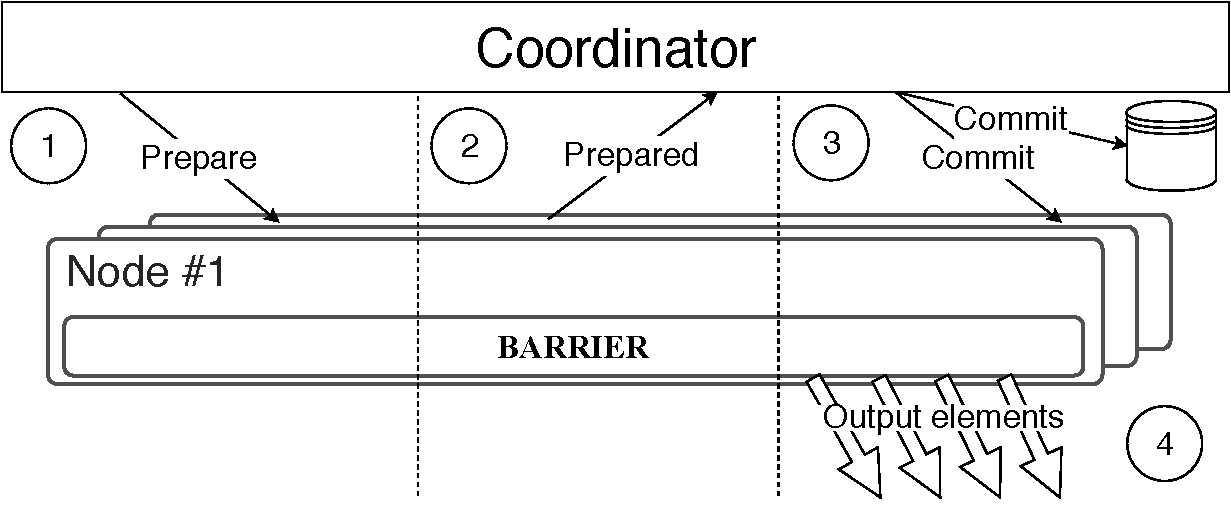
\includegraphics[width=0.42\textwidth]{pics/protocol-flink}
  \caption{State snapshotting protocol in Apache Flink}
  \label{protocol_flink}
\end{figure}

\begin{figure}[htbp]
  \centering
  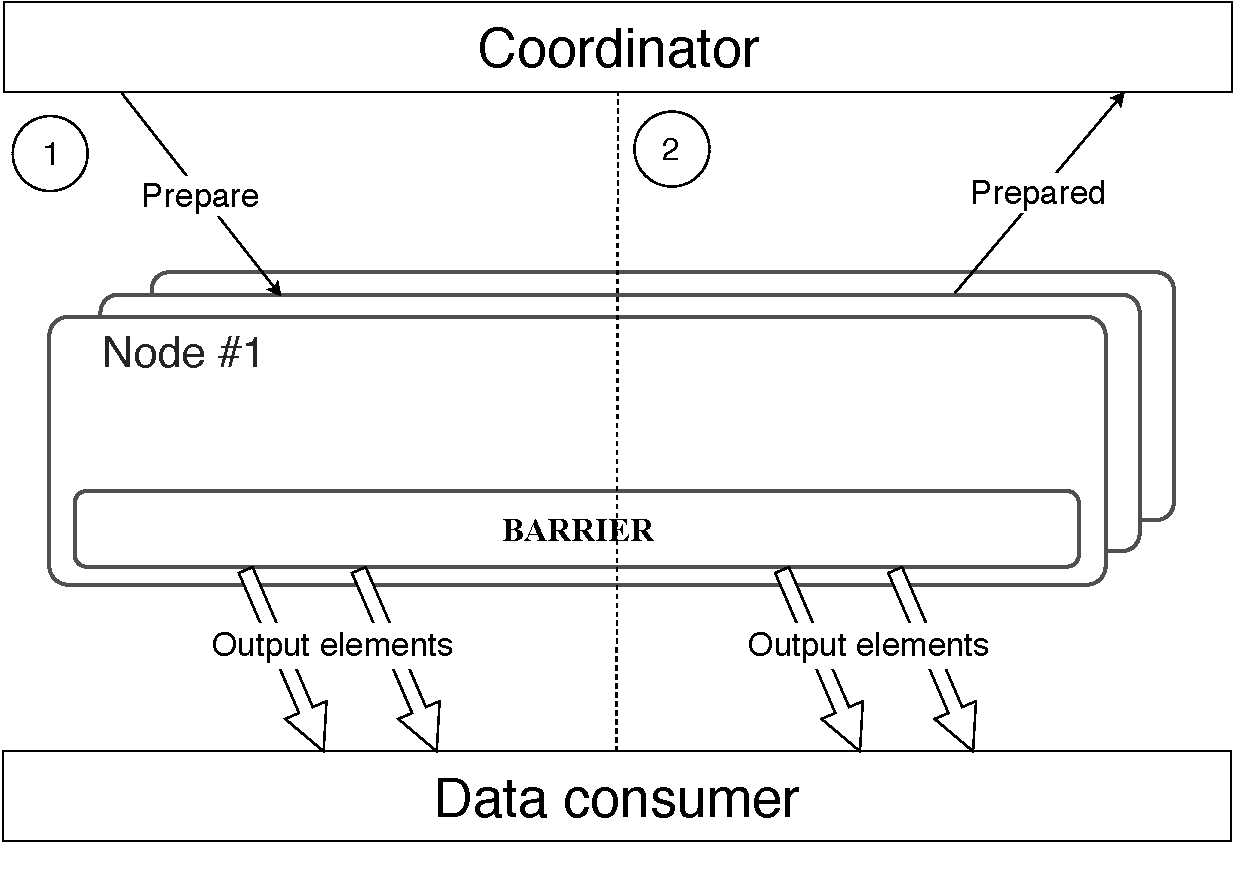
\includegraphics[width=0.42\textwidth]{pics/protocol-fs}
  \caption{State snapshotting protocol in a deterministic system}
  \label{protocol_fs}
\end{figure}

\subsubsection{Last output element}

In order to preserve the deterministic outcome, the Barrier must release output items with monotonically increasing $t(x)$. Hence, the Barrier can filter out any items with $t(x)$ less than or equal to the $t(x)$ of the last released item $t_{last}$ in order to preserve exactly-once after recovery. To implement this mechanism, there is a need to deliver output items and update $t_{last}$ atomically. To solve this problem, we require the following output protocol between a {\em barrier} and a {\em data consumer}: 

\begin{itemize}
    \item On each output delivery, Barrier sends a bundle to the data consumer. This bundle contains an output item and $t_{last}$. The Consumer must acknowledge that it received the bundle.
    \item Barrier does not send new output bundle until the previous one is not acknowledged.
    \item Consumer must return last received bundle on Barrier's request.
\end{itemize}

This protocol guarantees that $t_{last}$ and released items are always consistent with each other. It implies that the Barrier can request the last released bundle and fetch $t_{last}$ after recovery to avoid duplicates, which can be generated during input elements reprocessing.

Thus, on the one hand, we delegate the part of the basic functionality to data consumers. On the other hand, the requirement for a data consumer is not so strong and can be naturally satisfied by real-world consumers (HDFS, Kafka, databases, etc.). 

\subsection{Recovery}

Typically, distributed systems take into consideration the following types of failures:
\begin{itemize}
    \item Packet loss
    \item Node failure
    \item Network partitioning
\end{itemize}

Network partitioning is the particular case of failure because in this case, computations cannot be restarted. We believe that in this case, stream processing does not make sense. To the best of our knowledge, there are no open-source stream processing systems that tolerate network partitioning.

Failure detection can be implemented in different ways~\cite{hayashibara2002failure}, which are out of the scope of this paper. In~\FlameStream\ it is implemented using {\em Acker}~\cite{we2018adbis}. In the case of packet loss or node failure, a failure detector mechanism can enforce the Coordinator to begin computations restart from the last successful snapshot. Restart protocol includes the following steps:

\begin{itemize}
    \item Coordinator broadcasts a notification to begin the recovery process.
    \item Operations receive these notifications and fetch their states from state storage. After that, they send an acknowledgment that they are ready for Processing to the Coordinator.
    \item Barriers request the last released bundle from data consumers and send acknowledgments that they are ready for Processing to the Coordinator.
    \item When the Coordinator receives all acknowledgments from groupings and barriers, it requests data producer to replay starting from the $t(a)$ of the last snapshot.
\end{itemize}

The proposed protocol guarantees the following properties that allow preserving~ exactly-once:

\begin{itemize}
    \item Processing does not restart until all operations obtain consistent states. The consistency of these states is guaranteed by the state snapshotting protocol. Therefore, the elements are not lost.
    \item Duplicates are not produced because, at the moment when Processing is restarted, it is ensured that Barrier has obtained the last released $t(x)$ and can filter out extra items.
\end{itemize}